 \chapter{Data commonly used in species distribution models}
In total $34$ predictors are used. These predictors were selected because they are widely available and are often used in SDMs. Using $34$ predictors to build a species distribution model is rather 


\label{ch:DataCommonlyUsedInSpeciesDistributionModels}


\section{Predictor data}
To process the spatial data \texttt{R} is used as a geographic information system (GIS). To do this we rely on the \textsc{raster} \parencite{raster} and \textsc{sp} \parencite{sp} packages. Although this chapter is only a small piece of the thesis the data-preparation is the most labour intensive part of it. 


\subsection{Vegetation Continuous Fields}
The Vegetation Continuous Fields (\Citeauthor[VCF,][]{VCF}) data-set contains values between $0$ and $100$. These values lie in the interval $[0,100]$ and correspond to the proportional tree cover of the cell. Some cells also contain values larger than $100$ and these correspond to water or rasters with no available data. Since R has a \textsc{NA} value all the cells with values $> 100$ are set to \textsc{NA}. The raster is provided in the geogracphical coordinate system combined with the World Geodetic System 1984 datum (GCS\textunderscore WGS84). The resolution of the VCF raster is $0.002083$ decimal degrees.

\subsection{Bioclimatic variables}
The bioclimatic variables are a set of variables which describe ecologically relevant climate patterns. \todo[inline]{find a citation} The definition of each of the $19$ bioclimatic variables can be found in Table \ref{table:Bioclim}. The bioclimatic variables can be derived from monthly minimum, maximum, and average temperature and precipitation data.

\begin{table}[htb]
\centering
\begin{tabular}{ll}
\toprule
Variable name & Explanation \\ 
\midrule
BIO1 & Annual Mean Temperature \\
BIO2 & Mean Diurnal Range (Mean of monthly $\left( \text{Temp}_{max} - \text{Temp}_{min} \right)$ \\
BIO3 & Isothermality $\left( 100 \times \frac{\text{BIO2}}{\text{BIO7}} \right)$  \\
BIO4 & Temperature Seasonality $\left(SD(\text{Temp}_{avg}) \times 100\right)$ \\
BIO5 & Max Temperature of Warmest Month \\
BIO6 & Min Temperature of Coldest Month \\
BIO7 & Temperature Annual Range $\left(\text{BIO5} - \text{BIO6}\right)$ \\
BIO8 & Mean Temperature of Wettest Quarter \\
BIO9 & Mean Temperature of Driest Quarter \\
BIO10 & Mean Temperature of Warmest Quarter \\
BIO11 & Mean Temperature of Coldest Quarter \\
BIO12 & Annual Precipitation \\
BIO13 & Precipitation of Wettest Month \\
BIO14 & Precipitation of Driest Month \\
BIO15 & Precipitation Seasonality $\left( \right)$ \\
BIO16 & Precipitation of Wettest Quarter \\
BIO17 & Precipitation of Driest Quarter \\
BIO18 & Precipitation of Warmest Quarter \\
BIO19 & Precipitation of Coldest Quarter \\
\bottomrule
\end{tabular}
\caption{\label{table:Bioclim}Explanation of the bioclimatic variables.}
\end{table}

It is clear that the BIO05, BIO6, and BIO7 variables are linear dependent. This linear dependence can be problematic when using classification methods. It is interesting that for some of the methods that we introduce this will lead to no problems while it will for others. This will be discussed in more detail in Section \ref{sec:combinations}. \\ 

The monthly temperature and precipitation data was obtained from the PRISM database (\citeauthor{PRISM}). The PRISM rasters have a grid cell size of $0.00833$ degrees and the rasters are provided in the GCS\textunderscore WGS84 system. To calculate the bioclimatic variables we adapted the \textsc{biovars} function from the \textsc{dismo} package \parencite{dismo}. The \textsc{biovars} function from the \textsc{dismo} package does not allow the user to provide a layer of the mean temperature, instead it uses the average of the minimum and maximum temperature whenever the calculations require the mean temperature. Our adaptation does use the mean temperature layers and should be slightly more realistic.

\subsection{Normalized Difference Vegetation Index}
The Normalized Difference Vegetation Index (NDVI) is a measurement of the amount of vegetation. It is based on measurements of the reflectance of the infra-red and the near infra-red region. The NDVI takes on values between $-1$ and $1$ and high values correspond with live green vegetation. The NDVI raster used in this thesis originates form the Global Inventory Modeling and Mapping Studies (GIMMS) and is provided by the University of Maryland Global Land Cover Facility \parencite{pinzon2005satellite, tucker2005extended}. This database contain semi-monthly rasters of the NDVI value for the period 1983-2006. The original rasters had a cell-size of $0.07266$ decimal degrees. These rasters were originally \todo[inline]{cite paper Brody / Svenning on greenes in the US} resampled to $0.04166$ decimal degree rasters and the semi-monthly rasters were combined such that monthly rasters were obtained. To obtain an average monthly NDVI raster for each month the $24$ NDVI rasters were averaged. The $12$ resulting NDVI rasters are then used to calculate a minimum, maximum, and mean NDVI raster.

\subsection{Digital elevation model}
The digital elevation model (DEM) raster \parencite{DEM} contains data on the elevation throughout the US. It is the raster with the highest resolution, more specifically the cell size is $0.000833$ decimal degrees and the raster is provided in the GCS\textunderscore WGS84. The use of elevation in SDM is somewhat contested, see e.g.\ \cite{hof_usefulness_2012} and \cite{oke_distribution_2015}. However, since our main purpose is to test model selection techniques adding a potentially irrelevant predictor should not matter. Furthermore, it is often suggested that other variables directly derived from DEMs, e.g.\ slope, are more ecological relevant, however, to keep the amount of data in this thesis handleable we will restrict ourselves to the original raster.


\subsection{Land cover}
The land cover data is created from the National Land Cover Databases (NLCD) provided by the US Geological Survey. The NLCD are derived from landsat imagery of 2001 \parencite{vogelmann2001completion}, 2007 \parencite{homer2007completion}, and 2011 \parencite{fry2011completion}. These datasets were then transformed into rasters that utilize the Anderson level 1 classification \parencite{anderson_land_1976}. Eight different land cover classes are used: barren, forest, ice-snow, grassland, urban, water, wetlands, agriculture. For each class rasters with a cell size of $0.04166$ decimal degrees of the years 2001, 2007, and 2011 were created. In order to obtain one raster these were then averaged. The eight final rasters contain values in the interval $[0,1]$ and correspond to percentage of the respective land-cover within the cell. It is interesting that the sum of these rasters equals one, hence there is a linear dependence between the variables.

\subsection{Human Influence Index}
The Human Influence Index (\citeauthor{hii}) raster contains integer values between $0$ and $64$. High values indicate a strong human influence and vice versa. The index is derived from measures of the population density, the amount of roads, the amount of light sources during night-time, etc.\ The raster is reprojected to the GCS\textunderscore WGS84 spatial reference system and has a cell size of $0.00833$ decimal degrees.

\subsection{Preprocessing of the predictor data}

In order to speed up computations and facilitate general GIS operations the rasters are, if necessary, reprojected to the GCS\textunderscore WGS84 spatial reference system. The extent and resolution of the rasters is set to be equal to those of the DEM layer. This procedure makes sure that the cells of the rasters line up nicely. A visualization of the whole process can be found in Figure \ref{fig:DataCommonlyUsedInSpeciesDistributionModels:DataScheme}. Once all the data is preprocessed the rasters amount to over $300$ GB of data.

\begin{figure}[!htb]
\centering
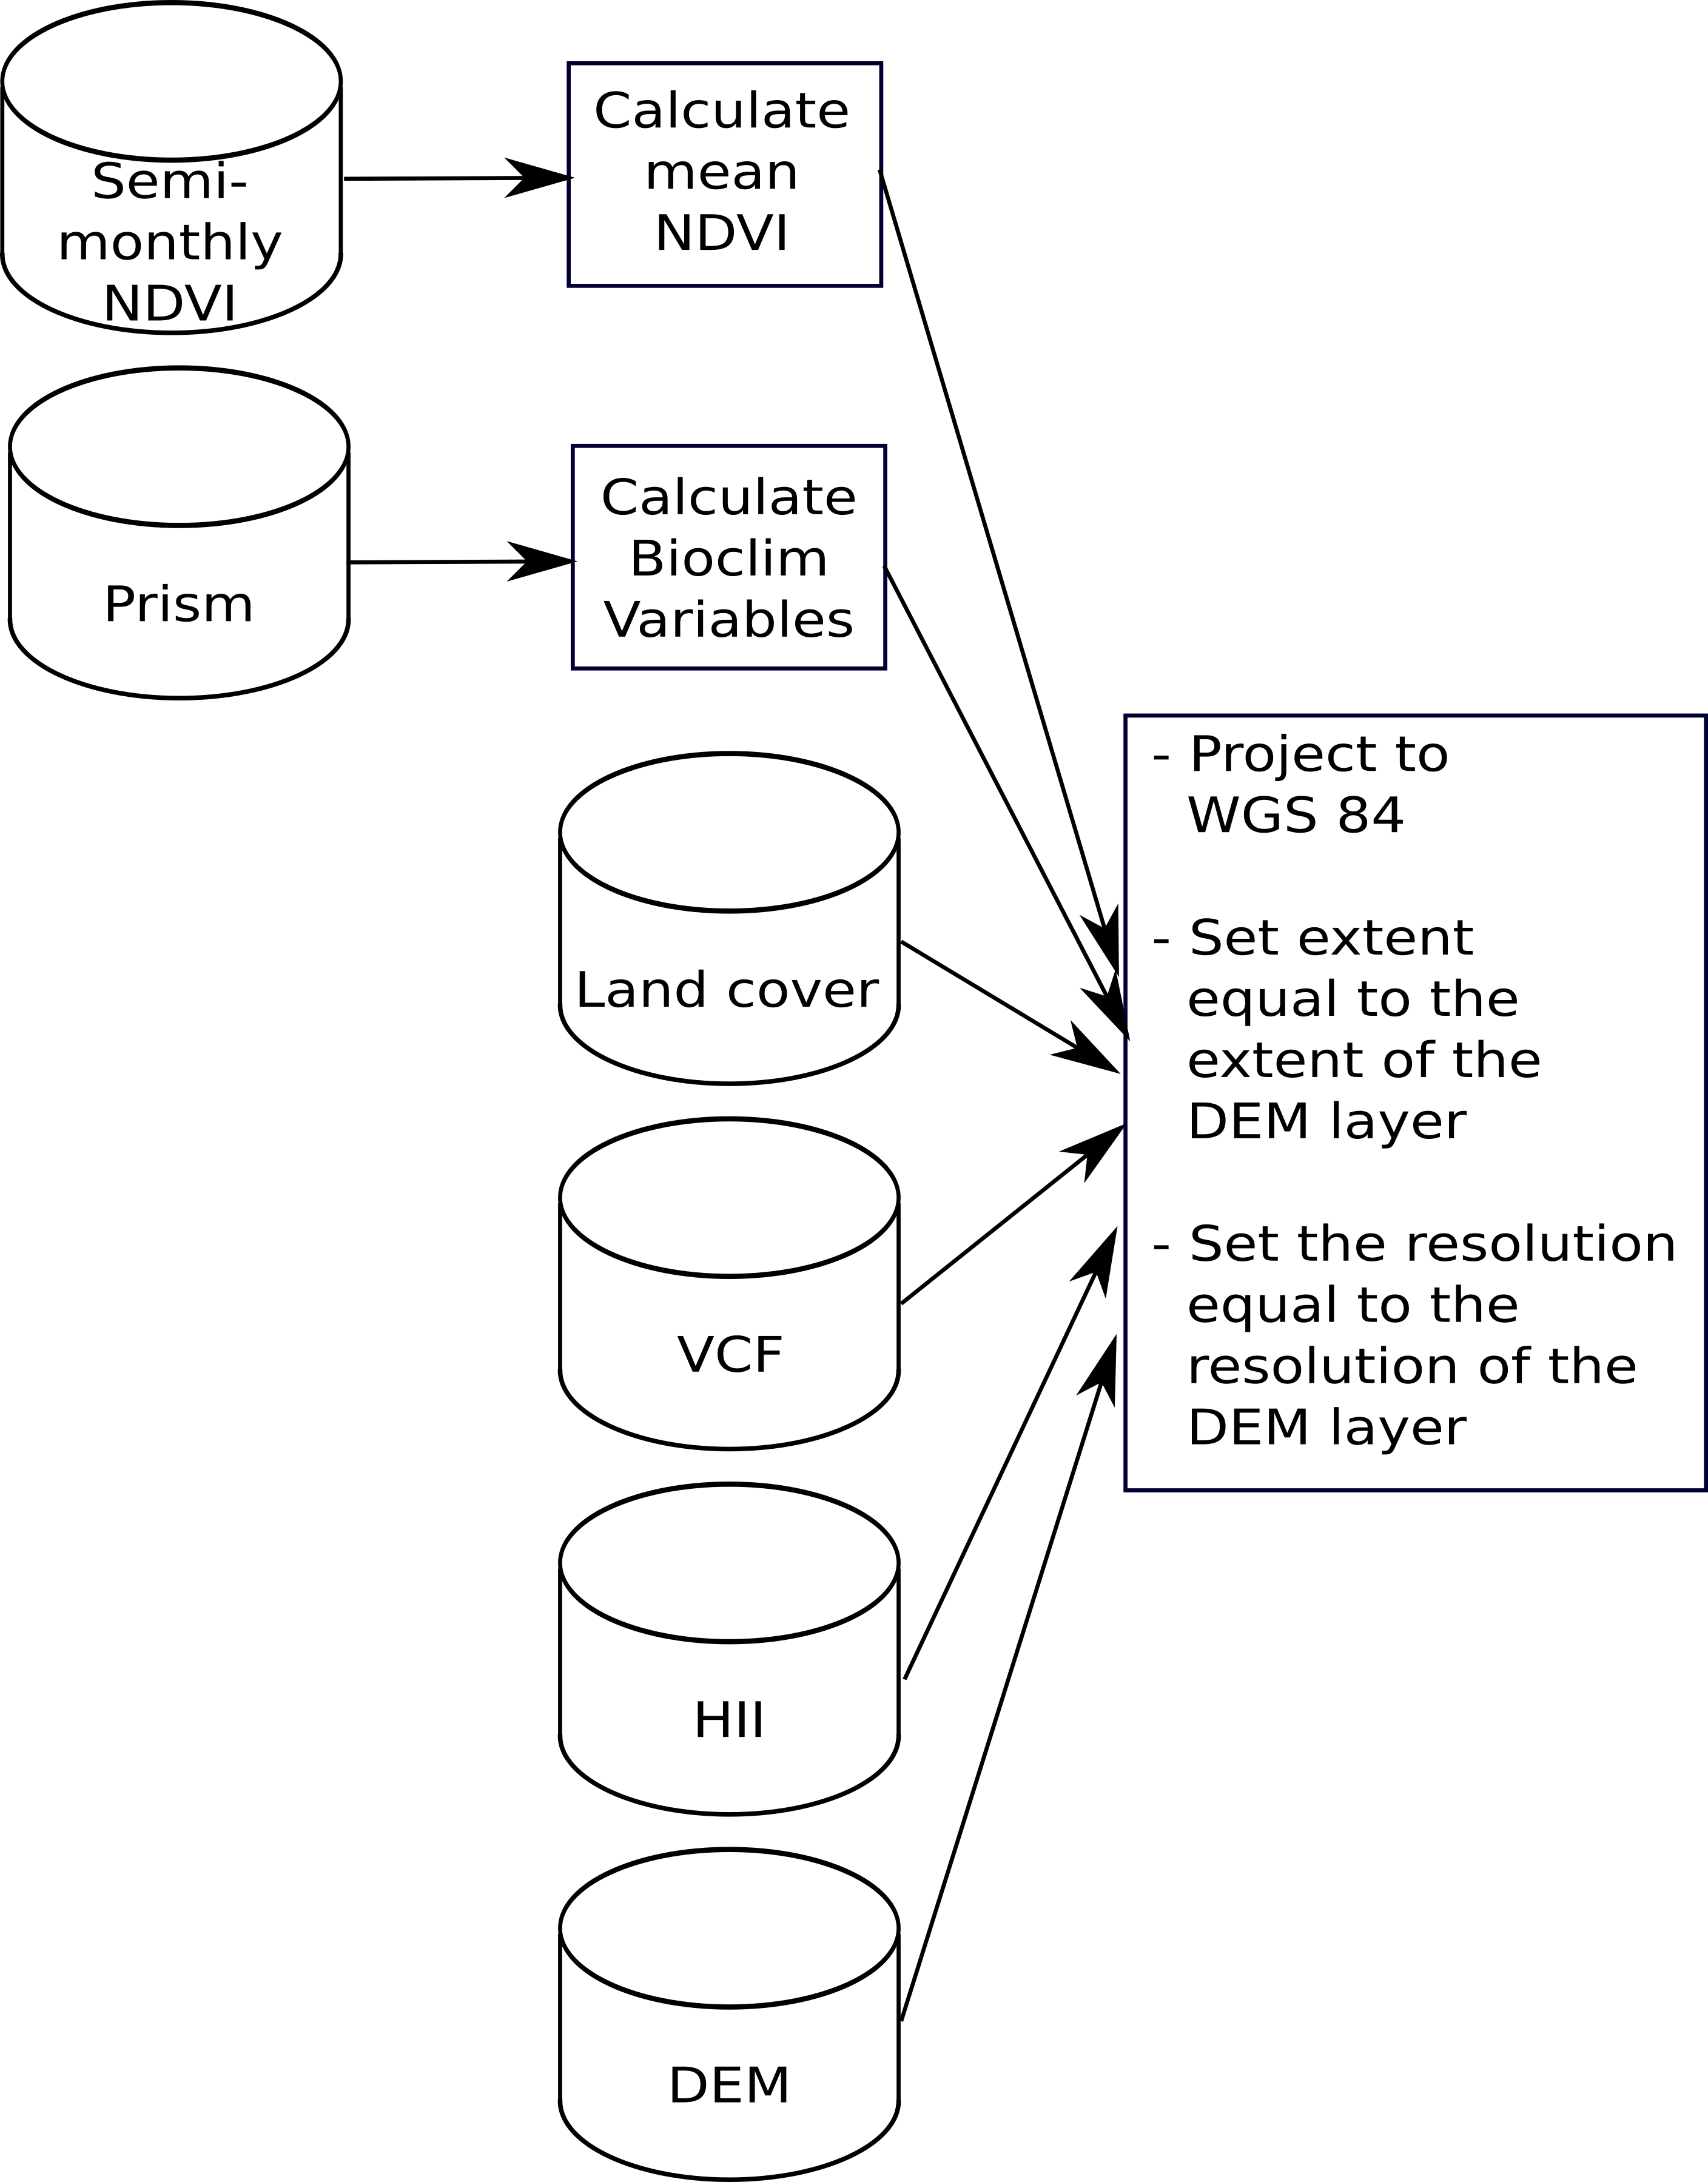
\includegraphics[scale=0.35]{VectorGraphics/DataScheme.png}
\caption{\label{fig:DataCommonlyUsedInSpeciesDistributionModels:DataScheme}Visualization of the preprocessing of the raster data.}
\end{figure}


\subsection{Exploratory analysis of the predictor data}
\label{sec:ExploratoryPredictor}

Since one would expect that the relationship between the variables is different in different geographical regions we defined four subregions of the contiguous United States. The regions and their defining bounding rectangles can be found in Figure \ref{fig:studyExtent}. \\


\begin{figure}[!htb]
\centering
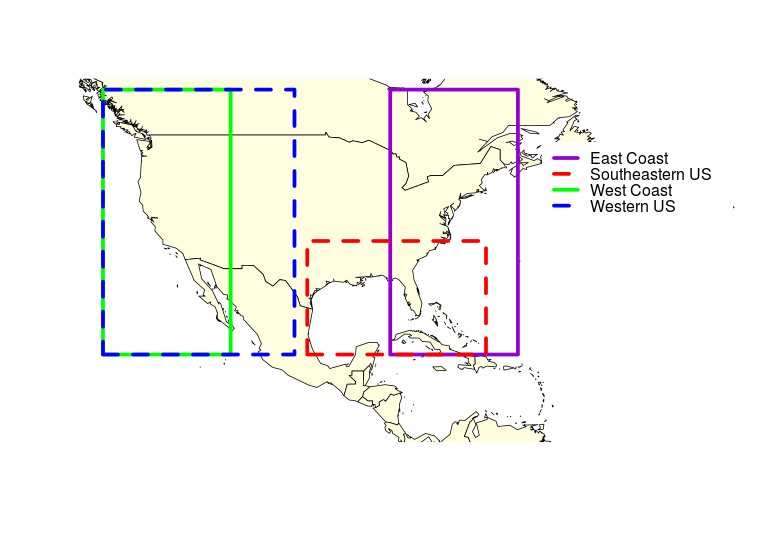
\includegraphics[scale=0.6]{Plots/StudyExtent.png}
\caption{\label{fig:studyExtent}Regions of the contiguous US and their bounding rectangles.}
\end{figure}

In order to check whether the relationship between the variables is different in different regions two sets of random points were generated, one with points within the contiguous United States and one that contains points within the West Coast region. For each point the corresponding values of the predictor rasters were extracted. Heat maps of the correlations of the predictor variables can be found in Figures \ref{fig:HeatBGUS} and \ref{fig:HeatBGWC}. A quick inspection of these plots learns that most correlations seem to be rather stable. There are however also some that change quite dramatically, e.g.\ the correlation between the ice-snow land cover class and the NDVI indices. Even though we only report the heat maps of the correlations for the US and the West Coast region similar behaviour could be observed for the other regions. \\

\begin{landscape}
\thispagestyle{empty}
\begin{figure}[!htb]
  \centering
  \makebox[\textwidth][c]{%
    \begin{minipage}{.90\textwidth}
    \centering
    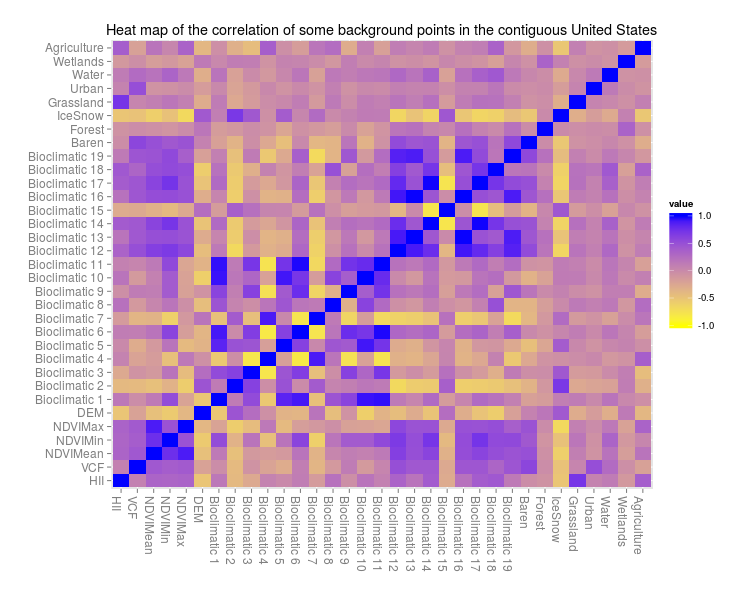
\includegraphics[width=\textwidth]{Plots/CorPlotUS.png}
    \caption{\label{fig:HeatBGUS}Heat map of the correlations in the US.}
    \end{minipage}
    \begin{minipage}{.90\textwidth}
    \centering
    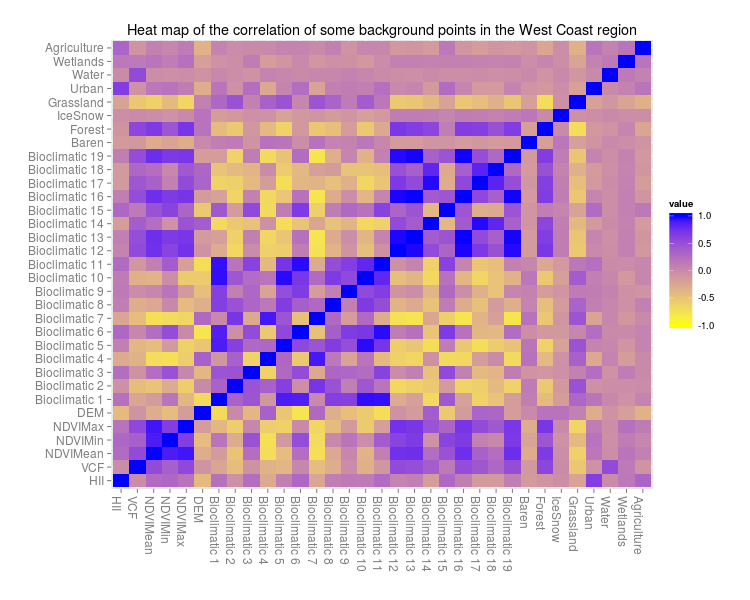
\includegraphics[width=\textwidth]{Plots/CorPlotBGWC.png}
    \caption{\label{fig:HeatBGWC}Heat map of the correlations in the West Coast region.}		\end{minipage}%
}
\end{figure}
\end{landscape}

It is interesting to note that the rank of the predictor data matrix of the random points is $32$. This is rather surprising since BIO7 is a linear combination of BIO5 and BIO6 and the land cover variables should sum to a constant hence one would expect that the rank is smaller or equal to $31$. A closer inspection leads to the conclusion that some small rounding errors in the creation of the land cover rasters ``remove'' the linear dependence. This ``near linear dependence'' also becomes clear when we look at the singular values of the scaled data matrix. The three smallest are $0.2139771, 0.000002,$ and $0$, for all practical purposes this means that there are two ``redundant'' variables.\\


\section{Outcome data}
\subsection{Species considered}
The species that will be studied can be found in Table \ref{table:Species}. These species were selected in such a way that different regions in the US are represented. This was done because, as we saw in Section \ref{sec:ExploratoryPredictor}, the relationship between the different predictors can be different in different regions. The extent of the species distribution is quite different across the selected species. For example the copperhead snake is spread throughout a large part of the US while the Sequoia sempervirens only occurs in a small strip of land stretching from Southern California to Southern Oregon. Having species for which the distribution within the study area is smaller or larger should lead to a different relationship between the predictors and the distribution. Finally, we included five plant and five animal species. This was done because it seems reasonable that the including fine grain predictors will lead to a larger increase in predictive performance of the classification models when the species is stationary.\\

\begin{sidewaystable}[!htb]
\centering
\begin{tabular}{l l c c c c c }
\toprule
Species & common name & US & West Coast & East Coast & Western US & Southeastern US \\
\midrule
Aesculus glabra & Ohio buckeye  &  \ding{51} \\
Juniperus osteosperma & Utah juniper  & & &  \ding{51}\\
Quercus ilicifolia & bear oak  & & &  \ding{51}  \\
Salix caroliniana & coastal plain willow  &  \ding{51}  \\
Sequoia sempervirens & coast redwood & &  \ding{51}  \\
\\
Agkistrodon contortrix Linnaeus & copperhead snake   &  \ding{51}  \\
Geomys pinetis Rafinesque & southeastern pocket gopher  &&&& &  \ding{51}  \\
Pituophis catenifer catenifer & Pacific gopher snake  &  &  \ding{51}  \\
Sorex pacificus & Pacific shrew &  &  \ding{51}  \\
Sylvilagus nuttallii & mountain cottontail  & & &  &  \ding{51}  \\
\bottomrule
\end{tabular}
\caption{\label{table:Species}The different species studied and the study extent.}
\end{sidewaystable}

\subsection{Global Biodiversity Information Facility}
The presence-only data originates from the Global Biodiversity Information Facility (GBIF) database. This database contains data from different other smaller occurrence only databases, e.g.\ data from citizen science projects (e.g.\ the iNaturalist project) or herbariums (e.g.\ The New York Botanical Garden Herbarium). These data sources are quite prone to errors. For example, citizen science data is usually provided by non-experts and misidentifications are quite likely. Even data collected by experts can be irrelevant for our purposes, for example herbarium data often includes observations in botanical gardens etc. Furthermore GBIF data tends to contain a lot of duplicated observations. Hence, before using the data from GBIF some data-cleaning was performed. Finally, because the predictors were recorded quite recently we decided to restrict ourselves to observations obtained from the 1980's onward. \\

\subsection{Forest Inventory and Analysis data}
The presence-absence data of the plant species was obtained from the The United States Forest Service Forest Inventory and Analysis (FIA) database. The data from this database consists of plot locations and all the tree species observed within each plot. The locations that are reported are, for privacy reasons, slightly distorted.\\ 

The sampling design that is used in the construction of this database changed in 1999 and details can be found in \cite{fiamanual}. By 2004 the new sampling design was implemented in nearly all the states of the contiguous US. The exceptions to this are New Mexico, Oklahoma, and Wyoming for which the new design was implemented in 2005, 2008-2009, and 2011. In each state at least 10\% of the plots is sampled each year, hence a time-frame of at least 10 years means that each plot site should be sampled. The time-frame that we use is 2004-2014, Since the sampling in New Mexico, Oklahoma, and Wyoming started later than 2004 these states are undersampled. Furthermore, states in the Easter US tend to have a sample intensity larger than 10\% and some plots were sampled multiple times. For the plots where this is the case we replace it with a new observation. If the plot contains the species of interest at least once the species is said to be present, otherwise it was absent in the plot. It might be interesting to use modelling methods that allow for a sampling design correct. However, this would lead is astray the sampling design will not be corrected for in this thesis.\\

Finally, the sampled plots are all contained within ``forested'' areas. This implies that lone standing trees will not be observed.

\subsection{data preparation}
In order to build the necessary models the predictor values corresponding to the presence or absence locations need to be extracted. For some of the locations some rasters contain a \textsc{NA} value. These points are removed before the models are constructed. This might lead to some slight biases in the models but since the goals is not to construct perfect interpretable models but to inspect the predictive performance this should not lead to large problems.
\section{Spatial scale}
\label{sec:SpatialScale}

\todo[inline]{cite Fine-scale environmental variation in species distribution modelling ...}